% fichier 'presentation.tex'
% auteur : Igor Milhit
% e-mail professionnel : igor.milhit@hesge.ch
% version 0.2
% cette présentation, sauf indication contraire, est sous licence CC-BY

\documentclass[12pt]{beamer}
\mode<presentation> {
	\usetheme{Hannover} 
	\usecolortheme{seagull} 
%	\setbeamercovered{transparent}
	
	}

\usepackage[french]{babel}
\usepackage[utf8]{inputenc}
\usepackage{lmodern}
\usepackage[T1]{fontenc}
\usepackage{url}
\usepackage{soul}


\logo{
\includegraphics[width=1.9cm]{heg-logo.jpg}}
\setbeamertemplate{navigation symbols}{}


\title[La sécurité]
{La sécurité}
\subtitle {HEG-ID --- Infobase}

\author[AB / IM / RR]
{Alexandre~Boder \and Igor~Milhit \and Raphael Rey}
\institute[Haute École de Gestion de Genève] % (facultatif mais généralement nécessaire)
{Haute École de Gestion de Genève\\Filière Information Documentaire}
\titlegraphic{

\includegraphics[scale=.2]{heg-logo.jpg}\hspace{.2cm}
}

\date[2014]{2014}
\subject{Sécurité des systèmes d'information}
\keywords{SSI, sécurité, système d'information}




% À supprimer si vous ne voulez pas que la table des matières apparaisse
% au début de chaque sous-section :
 \AtBeginSection[] {
	\begin{frame}<beamer>{Structure}
		\begin{center}
		 \tableofcontents[currentsection,hideothersubsections]
		\end{center}
	\end{frame}
}


\begin{document}

% page de titre
	\begin{frame}
		\titlepage
	\end{frame}
	
	\begin{frame}{La sécurité ?}
		\begin{itemize}
			\onslide<1>\item Qu'est-ce que \alert{la sécurité} vous évoque ?
			\onslide<2->\item \href{http://www.informationisbeautiful.net/visualizations/worlds-biggest-data-breaches-hacks/}{{\color{blue}Worlds biggest data breaches hacks}}
			% Attention, les liens suivants sont morts, d'ailleurs parce que le site a à nouveau été hacké
			\onslide<3->\item \href{http://annelaurejacquart.com/2013/11/le-site-est-mort-vive-le-site/} {{\color{blue}\st{Le site est mort, vive le site !}}} et \href{https://www.mavenhosting.com/clients/announcements.php?id=8}{{\color{blue}\st{mavenhosting}}}
			\onslide<4->\item \href{http://reflets.info/a-propos-des-journees-portes-ouvertes-du-groupe-ump-au-senat/}{{\color{blue}Journée portes ouvertes du groupe UMP au Sénat}}
		\end{itemize}
	\end{frame}

% page de table des matières.
	\begin{frame}{Plan}
		\tableofcontents[pausesections,hideallsubsections]
		% Vous pouvez, si vous le souhaiter ajouter l'option [pausesections]
		% Ici l'option [hideallsubsections] pour n'afficher que les sections dans la toc
	\end{frame}

%%%%%%%%%%%%%%%
%% Section 1 %%
%%%%%%%%%%%%%%%

\section{Identification / Authentification}

	\subsection{Définitions}
		
		\begin{frame}{Identification}
			\onslide<1->
			\begin{exampleblock}{Définition}
				"[...] en informatique, l'\alert{identification} permet de connaître l'identité d'une entité, 
				souvent à l'aide d'un identifiant tel qu'un nom d'utilisateur." (Wikipédia)
			\end{exampleblock}
			\onslide<2>
			\begin{itemize}
				\item Nom, prénom
				\item Pseudo, nickname
				\item Adresse e-mail
				\item Biométrie ?
			\end{itemize}
		\end{frame}
		
		\begin{frame}{Authentification}
			\onslide<1->
			\begin{exampleblock}{Définition}
				"L'\alert{authentification} est la procédure qui consiste, pour un système informatique, 
				à vérifier l'identité d'une personne ou d'un ordinateur afin d'autoriser l'accès de cette entité 
				à des ressources [...]." (Wikipédia)
			\end{exampleblock}
			\onslide<2>
			\begin{itemize}
				\item mot de passe
				\item passphrase
				\item carte d'identité, passeport
			\end{itemize}
		\end{frame}
		
	\subsection{Fonctions}
		
		\begin{frame}{Identification}{Ordinateur personnel}
			\begin{itemize}
				\item Administrateur
				\item Utilisateur 1
				\item Utilisateur 2
				\item Visiteur
				\item ...
			\end{itemize}
		\end{frame}
		
		\begin{frame}{Identification}{Ordinateur personnel}
			\onslide<1->
			\begin{exampleblock}{Question}
				Que peut-on faire en accédant à votre ordinateur personnel, avec votre session ouverte ?
			\end{exampleblock}
			\onslide<2>
			\begin{itemize}
				\item Accéder aux données
				\item Aux mots de passes du navigateur
				\item $\rightarrow$ Aux comptes en lignes
				\item e-mail
				\item Droits d'administration (installation...)
			\end{itemize}
		\end{frame}
		
	\subsection{Mot de passe}	
		
		\begin{frame}{Des idées ?}
			\begin{exampleblock}{Question}
				Qu'est-ce qu'un bon mot de passe ?
			\end{exampleblock}
		\end{frame}
		
		\begin{frame}{Règles}{création}
			\begin{itemize}
				\item Pas de mot de dictionnaire ou de nom propre
				\item Pas de date, de numéro postal ou d'année
				\item 8 caractères au minimum
				\item alphabet, minuscule, majuscule, chiffre, caractères spéciaux
				\item passphrase
				\item aléatoire
			\end{itemize}
		\end{frame}
		
		\begin{frame}{Règles}{gestion}
			\begin{itemize}			
				\item \alert{NE JAMAIS DIVULGUER}
				\item Ne pas les écrire
				\item Ne pas le communiquer par e-mail
				\item Ne pas utiliser 2x le même mot de passe
				\item Changer régulièrement
				\item Gestionnaire de mot de passe : Keepass \url{http://keepass.info/} \\
					Lastpass \url{https://lastpass.com/}
			\end{itemize}
		\end{frame}
		
		\begin{frame}{Protection}
			\begin{exampleblock}{Question}
				Est-ce que le mot de passe est suffisant ?
			\end{exampleblock}			
		\end{frame}


%%%%%%%%%%%%%%%
%% Section 2 %%
%%%%%%%%%%%%%%%

\section{Sécurité des données}

	\subsection{Sauvegardes}
	
		\begin{frame}{Définitions}{sauvegarde}
			\begin{exampleblock}{Définition}
				"En informatique, la \alert{sauvegarde} (backup en anglais) est l'opération qui consiste à dupliquer 
				et à mettre en sécurité les données contenues dans un système informatique." (Wikipédia)
			\end{exampleblock}	
			\begin{itemize}
				\item $\neq$ enregistrement
				\item $\neq$ archivage
				\item $\neq$ synchronisation
				\item \textit{Quid} du cloud ?
			\end{itemize}		
		\end{frame}
		
		\begin{frame}{Définitions}
			\begin{exampleblock}{Définitions}
				\alert{Externe} : la sauvegarde doit être faite sur un support indépendant du système informatique concerné \\
				\alert{Distante} : la sauvegarde peut être réalisée sur un support situé dans un lieu indépendant, par exemple via le réseau
			\end{exampleblock}
		\end{frame}
		
		\begin{frame}{Distante}{difficultés}
			\begin{itemize}
				\item Connexion sécurisée
				\item Données chiffrées
			\end{itemize}		
		\end{frame}
		
		\begin{frame}{Définitions}{types de sauvegardes}
			\begin{exampleblock}{Définitions}
				\alert{Complète} : "consiste à copier toutes les données à sauvegarder que celles-ci soient récentes, anciennes, modifiées ou non." (Wikipédia) \\
				\alert{Différentielle} : copie uniquement ce qui a changé depuis la dernière sauvegarde complète \\
				\alert{Incrémentale} : copie uniquement ce qui a changé depuis la dernière sauvegarde différentielle
			\end{exampleblock}
		\end{frame}
		
		\begin{frame}{Définition}{restauration}
			\begin{exampleblock}{Définition}
				La \alert{restauration} consiste à rétablir les données à partir des sauvegardes. La méthode et les possibilités dépendent notamment du type
				de sauvegarde utilisé.
			\end{exampleblock}
		\end{frame}

	\subsection{Chiffrement}
	
		\begin{frame}{Définitions}
			\begin{exampleblock}{Définitions}
				\alert{Crypter, cryptage, etc.} : n'existent pas en français  \\
				\alert{Chiffrer} : "transcrire des messages en un langage secret." (TLFi) \\
				\alert{Déchiffrer} : transcrire en langage clair un message codé, en possédant la clé \\
				\alert{Décrypter} : décoder un message sans connaître la clé
			\end{exampleblock}
		\end{frame}
		
		\begin{frame}{Définitions}
			\begin{exampleblock}{Définitions}
				\alert{Algorithme} : suite de processus, ou d'étapes permettant de chiffrer/déchiffrer\\
				\alert{Clé de chiffrement} : un des paramètres de l'algorithme, sur lequel repose la sécurité du chiffrement
			\end{exampleblock}
		\end{frame}
		
		\begin{frame}{Chiffres}
			\begin{columns}
				\begin{column}[c]{5cm}
					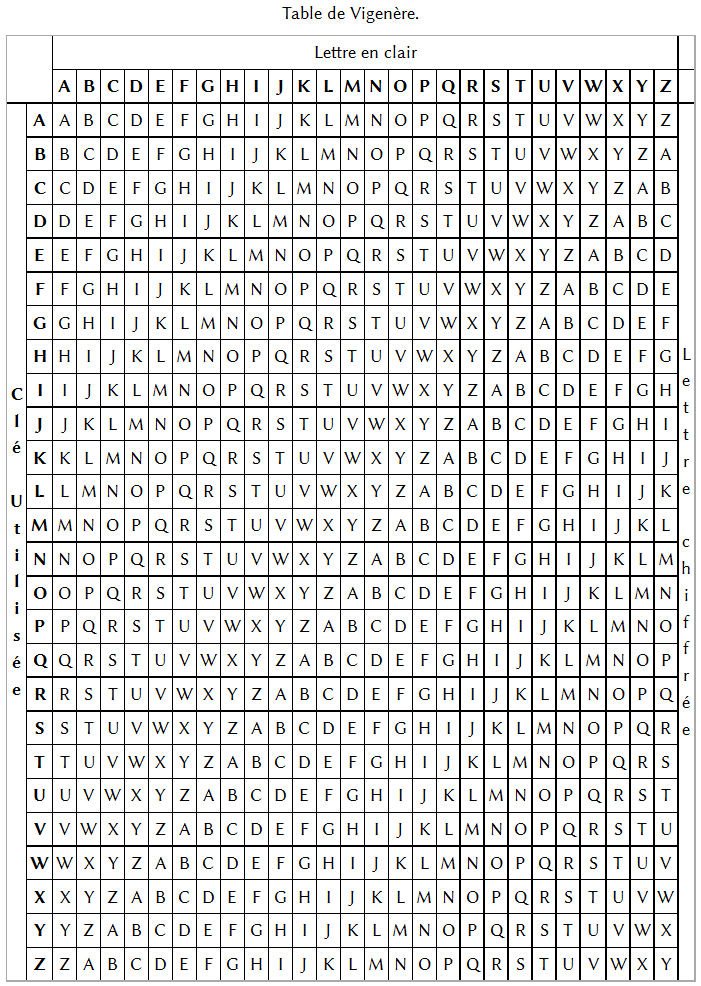
\includegraphics[scale=0.26]{table_vigenere.png}\\{\footnotesize Source: Wikipedia}
				\end{column}
				\begin{column}[c]{5cm}
					\begin{itemize}
						\item Chiffre de César
						\item Chiffre de Vigenère
					\end{itemize}
				\end{column}
			\end{columns}		
		\end{frame}
		
		\begin{frame}{Méthodes}{Symétrie}
			\begin{center}
				\onslide<1-> 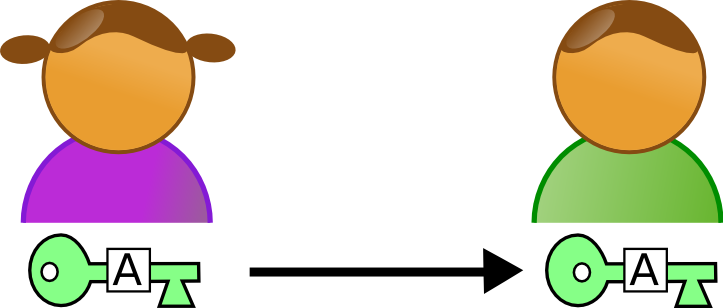
\includegraphics[scale=.28]{symetric_cryptography_-_step_1.png}\vspace{.2cm}\\
				\onslide<2> \hspace{.5cm}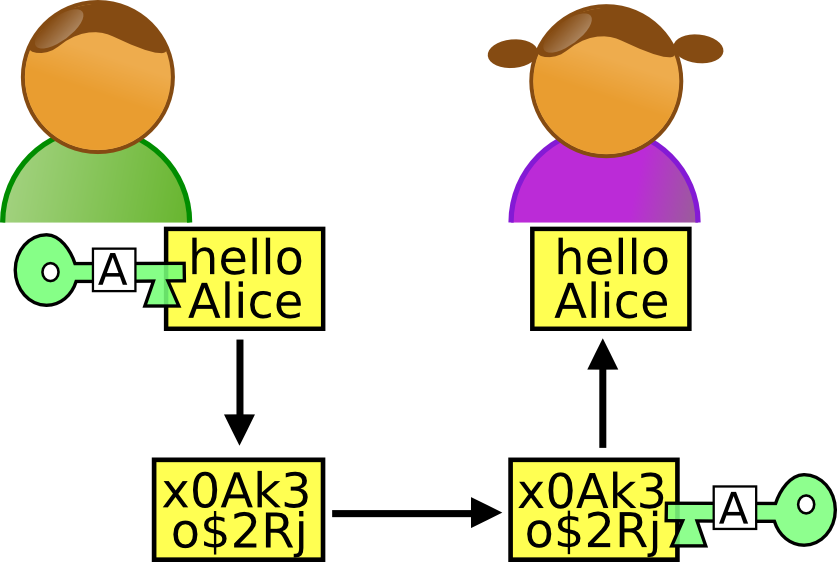
\includegraphics[scale=.26]{symetric_cryptography_-_step_2.png}			
			\end{center}
		\end{frame}
		
		\begin{frame}{Méthodes}{Asymétrie}
			\begin{center}
				\onslide<1-> 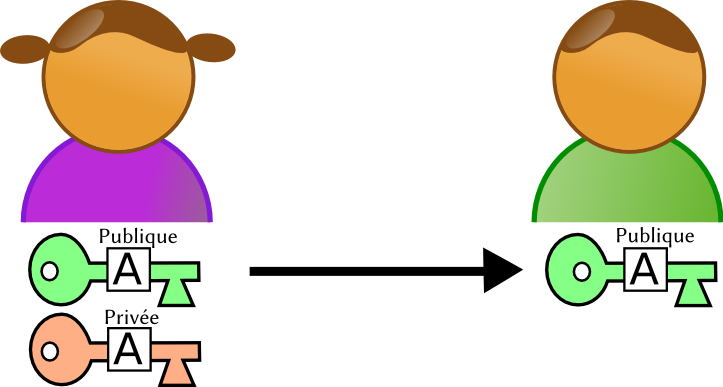
\includegraphics[scale=.28]{Asymetric_cryptography_-_step_1.png}\vspace{.1cm}\\
				\onslide<2> \hspace{.5cm}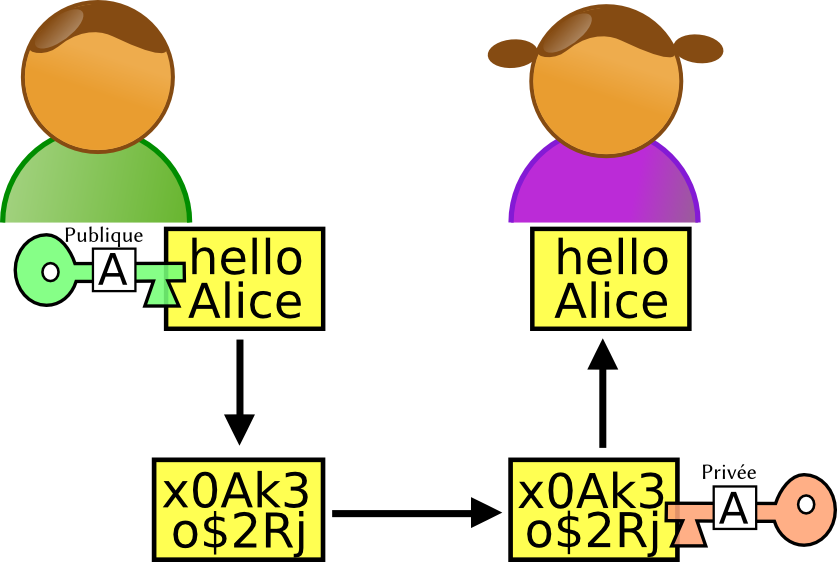
\includegraphics[scale=.26]{Asymetric_cryptography_-_step_2.png}
			\end{center}
		\end{frame}
		
		\begin{frame}{Utilisations}
			\begin{itemize}
				\item Communications chiffrées
					\begin{itemize}
						\item e-mail
						\item Instant Messaging
						\item VoIP
					\end{itemize}
				\item Connexions chiffrées
					\begin{itemize}
						\item HTTPS
						\item VPN
					\end{itemize}	
				\item Données chiffrées
					\begin{itemize}
						\item Fichier
						\item Répertoire
						\item Partition (Disque)
						\item Données stockées sur les serveurs d'autrui ("cloud")
					\end{itemize}
			\end{itemize}
		\end{frame}
		
		\begin{frame}{Fonction de hashage}
			\onslide<1->
			\begin{exampleblock}{Définition}
				 "On nomme \alert{fonction de hachage} une fonction particulière qui, à partir d'une donnée fournie en entrée, 
				calcule une empreinte servant à identifier rapidement, bien que incomplètement, la donnée initiale." (Wikipedia)
			\end{exampleblock}
			\onslide<2>
			\begin{center}
				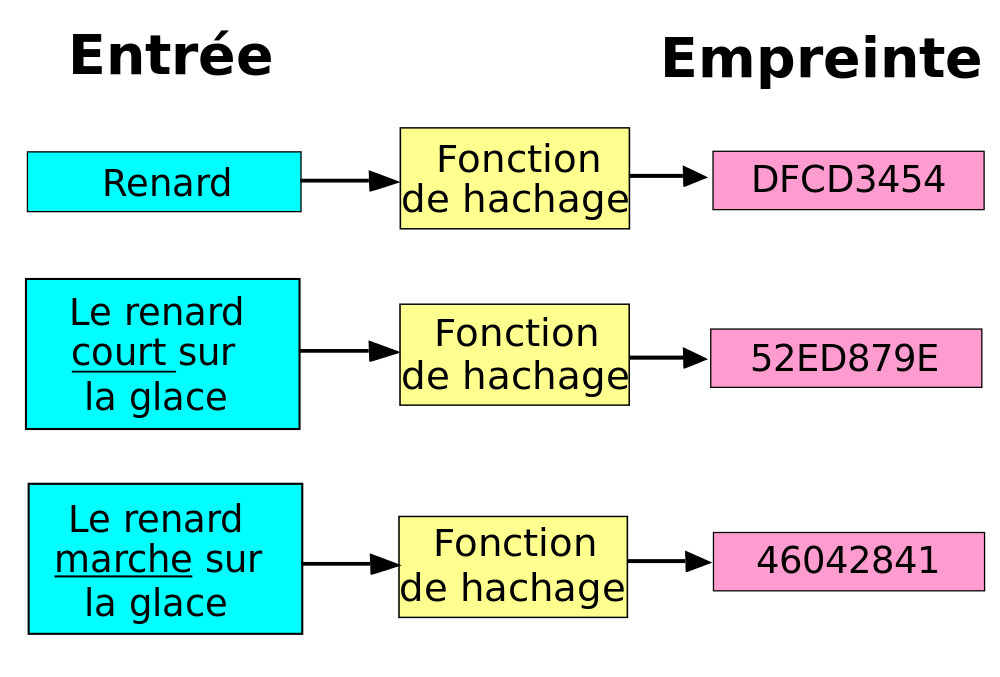
\includegraphics[scale=.21]{Hash_function_fr.png}
			\end{center}
		\end{frame}
		
		\begin{frame}{Signature}
			\begin{exampleblock}{Définition}
				Technique informatique qui permet d'assurer l' \alert{intégrité} et l' \alert{authenticité} d'un document électronique, au moyen de la fonction de hashage et du chiffrement.
			\end{exampleblock}
		\end{frame}
		
% 		\begin{frame}{}
% 			\begin{center}
% 				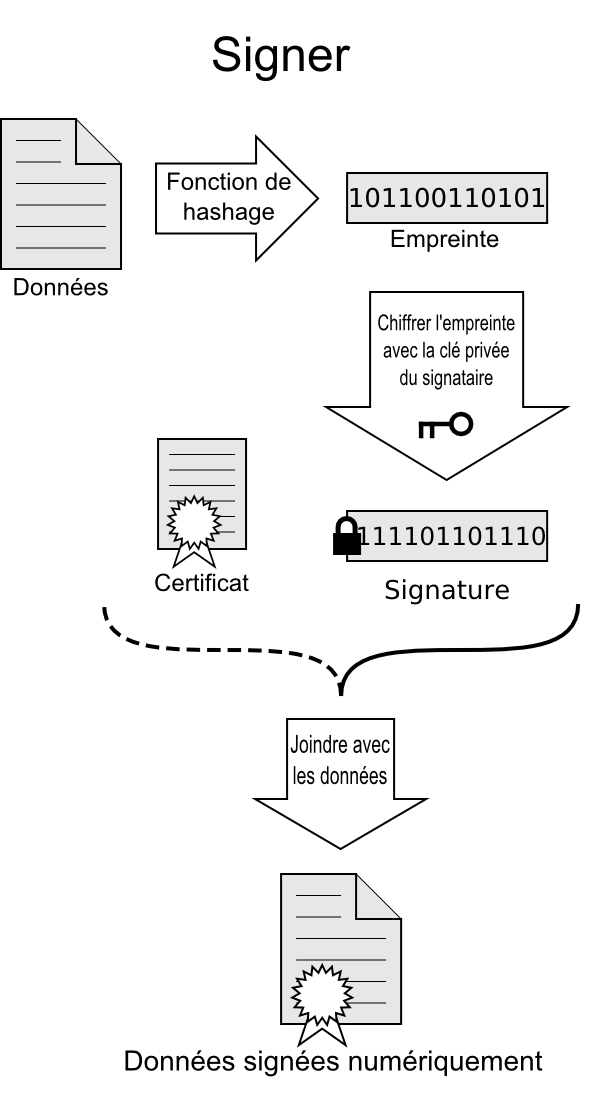
\includegraphics[scale=.3]{Digital_Signature_diagram_01.png}
% 			\end{center}
% 		\end{frame}
% 		
% 		\begin{frame}{}
% 			\begin{center}
% 				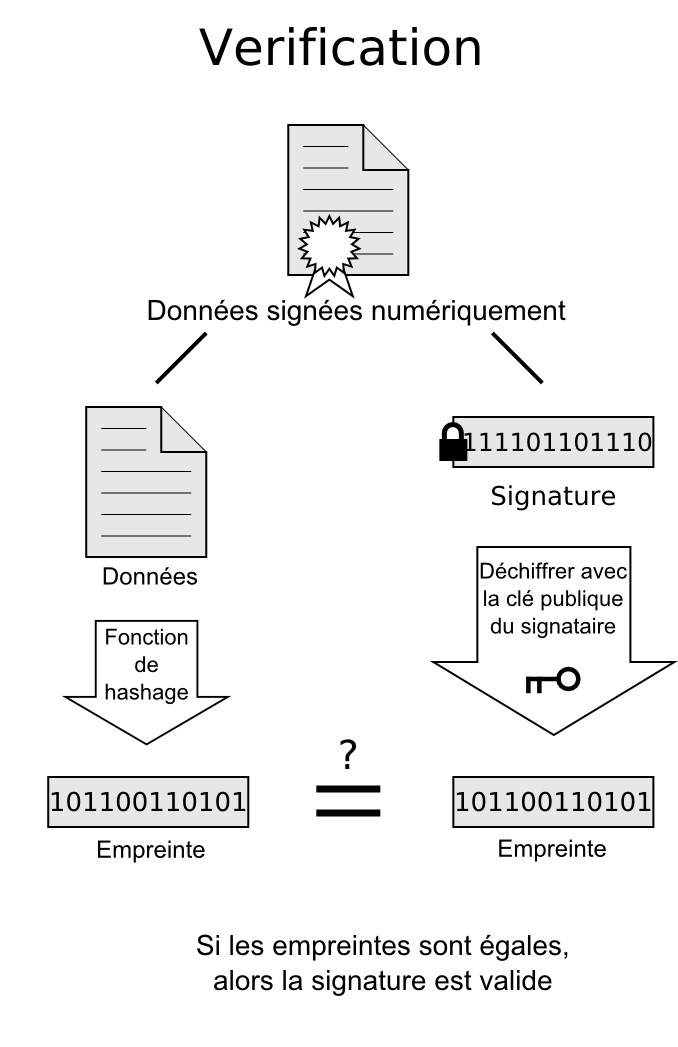
\includegraphics[scale=.3]{Digital_Signature_diagram_02.png}
% 			\end{center}
% 		\end{frame}

%%%%%%%%%%%%%%%
%% Section 3 %%
%%%%%%%%%%%%%%%

\section{Menaces}
	
	\subsection{Logiciels Malveillants}
	
		\begin{frame}{Adwares}
			\begin{exampleblock}{Définition}
						Un \alert{Adware}, ou \alert{publiciel} est un logiciel qui insère de la publicité à l'installation, par exemple sous la forme d'une barre d'outil ou de la configuration d'un moteur de recherche "exotique" par défaut.
				\end{exampleblock}		
		\end{frame}
		
		\begin{frame}{Virus}
			\begin{exampleblock}{Définitions}
						Un \alert{virus} est un programme qui se réplique lui-même, avec pour but de se propager d'un ordinateur à l'autre au moyen d'un "hôte", le plus souvent un logiciel.
				\end{exampleblock}		
		\end{frame}
		
		\begin{frame}{Ver}
			\begin{exampleblock}{Définition}
						Contrairement au virus, le \alert{ver} n'a pas besoin d'"hôte" pour se reproduire et se propager. 
				\end{exampleblock}		
		\end{frame}
		
		\begin{frame}{Cheval de Troie}
			\begin{exampleblock}{Définition}
						Un \alert{cheval de Troie} est un logiciel d'apparence légitime qui, en plus des fonctions attendues par l'utilisateur, exécute des fonctions sans que l'utilisateur s'en aperçoive. (Wikipedia)
				\end{exampleblock}		
		\end{frame}
		
		\begin{frame}{Spywares}
			\begin{exampleblock}{Définition}
						Un \alert{logiciel espion} ou \alert{mouchard} est comme son nom l'indique un  logiciel qui a pour objectif d'intercepter l'activité d'un utilisateur, le plus souvent dans un contexte d'espionnage industriel.
				\end{exampleblock}		
		\end{frame}		
		
		\begin{frame}{Keylogger}
			\begin{exampleblock}{Définition}
						Un \alert{keylogger} (ou enregistreur de frappe) est un logiciel qui peut enregistrer l'activité du clavier et peut donc être utilisé pour intercepter les mots de passe ou dans un but d'espionnage industriel.
				\end{exampleblock}		
		\end{frame}
		
		\begin{frame}{Porte dérobée}
			\begin{exampleblock}{Définition}
					Une \alert{porte dérobée}, ou \alert{backdoor} est une fonctionnalité inconnue de l'utilisateur qui donne accès à un utilisateur externe au logiciel, voire au hardware.
			\end{exampleblock}		
		\end{frame}
	
	\subsection{Autres menaces}
	
		\begin{frame}{Hameçonnage}
			\begin{exampleblock}{Définition}
				Le \alert{hameçonnage} ou le \alert{phishing} consiste à diriger un internaute sur un site web leurre, afin de lui soutirer des informations confidentielles
			\end{exampleblock}
		\end{frame}
		
		\begin{frame}{Ingénierie sociale}
			\begin{exampleblock}{Définition}
				L'\alert{ingénierie sociale} est une technique d'attaque qui ne repose pas sur des moyens technologique mais sur les comportements humains.
			\end{exampleblock}
		\end{frame}	
		
	\subsection{Objectifs}	
	
		\begin{frame}
			Les \alert{logiciels malveillants} ont pour objectifs :
				\begin{itemize}
					\item d'accéder aux données et/ou les détruire
					\item d'accéder au système informatique et/ou le détruire
					\item d'utiliser le système informatique pour :
						\begin{itemize}
							\item diffuser des virus
							\item envoyer des spams
							\item attaquer d'autres systèmes informatique (ex: DDOS)
						\end{itemize}
				\end{itemize}
		\end{frame}
		
	\subsection{Protection}
	
		\begin{frame}{Anti-virus}
			\begin{exampleblock}{Définition}
				Un \alert{anti-virus} est un logiciel qui identifie, isole ou détruit un virus.
			\end{exampleblock}
		\end{frame}

		\begin{frame}{Pare-feu}
			\begin{exampleblock}{Définition}
				Un \alert{pare-feu} ou \alert{firewall} est un système qui empêche les accès non autorisés depuis un réseau privé, ou à partir d'un réseau privé. (\url{https://wiki.debian.org/Firewalls})
			\end{exampleblock}
		\end{frame}
		
		\begin{frame}{}
			\begin{center}
				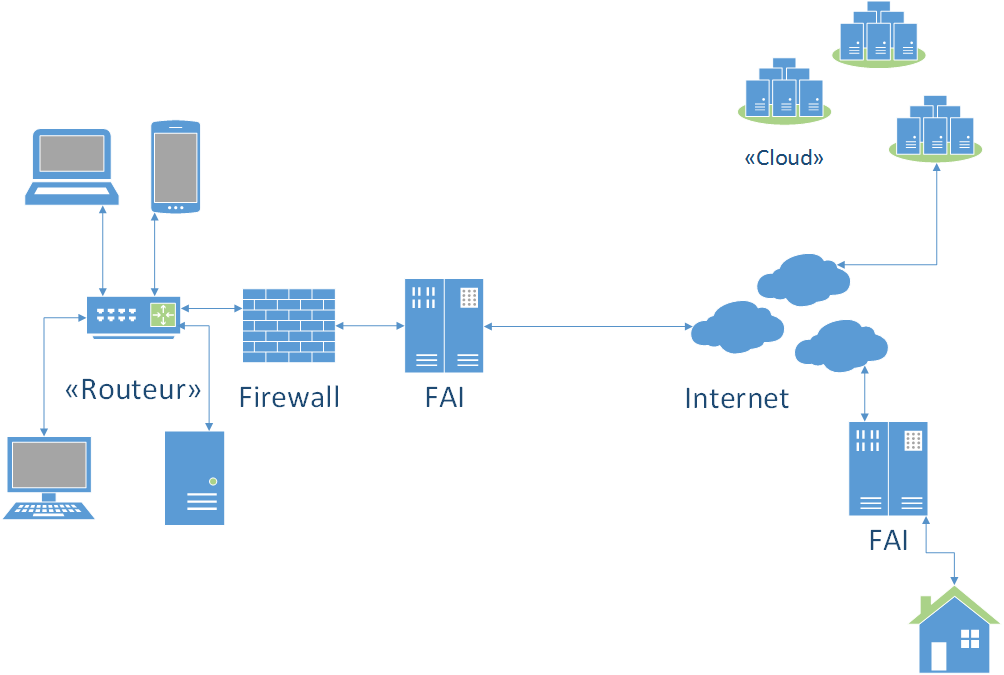
\includegraphics[scale=.35]{LAN-WAN.png}
			\end{center}
		\end{frame}

%%%%%%%%%%%%%%%
%% Section 4 %%
%%%%%%%%%%%%%%%

\section{SSI}
	
	\subsection{Définitions}

		\begin{frame}{SSI}
			\begin{exampleblock}{Définition}
				La \alert{sécurité des système d'information (SSI)} comprend l'ensemble des moyens pour garantir la protection d'un système d'information.
			\end{exampleblock}
		\end{frame}
		
		\begin{frame}{Données}

			\onslide<1->\begin{exampleblock}{Intégrité}
				\begin{itemize}
					\item des données : les données ne doivent pas être détruites ou altérées de manière non autorisée.
					\item du système : le système doit faire ce qu'on lui demande sans modification non autorisée.
				\end{itemize}
			\end{exampleblock}
			\onslide<2->\begin{exampleblock}{Disponibilité}
				Les données doivent être accessible en tout temps. Ou, du moins, de manière satisfaisante pour les besoins.
			\end{exampleblock}
		\end{frame}
		
		\begin{frame}{Transactions}
			\onslide<1->\begin{exampleblock}{Confidentialité}
				L'information ne doit être accessible et diffusée que par les personnes autorisées.
			\end{exampleblock}
			\onslide<2>Contexte des bibliothèques ? \\
			\onslide<3>\href{https://id-libre.org/shaarli/?aUbIGw}{{\color{blue}Adobe Digital Edition 4.0}}
		\end{frame}
		\begin{frame}{Transactions}
			\begin{exampleblock}{Authentification}
				Les acteurs doivent être identifiés et authentifiés, afin d'assurer la loyauté des transactions.
			\end{exampleblock}
		\end{frame}
	
	\subsection{Risques}
	
		\begin{frame}{Types de risques}
			\begin{itemize}
				\item Protection de la vie privée
				\item Responsabilité civile et/ou pénale
				\item e-Réputation, confiance
				\item Pertes financières
			\end{itemize}
		\end{frame}

\end{document}
